\documentclass[a4,11pt,
%notes,
slidesonly,
portrait,
fleqn]{seminar}

\slideframe{empty}

\slidesmag{2}

\usepackage{graphicx}
\pagestyle{empty}
\begin{document}
\begin{slide*}
  \section*{Relational Databases Theory and Logic}
The following slides provide a first logic oriented view to relational
database theory. It is not very feasible in practice! 

Better methods will be discussed as the course proceeds.

(Thanks to Prof.\ Enrico Franconi, University Bozen-Bolzano, 
for the following slides)
\end{slide*}
\begin{slide*}
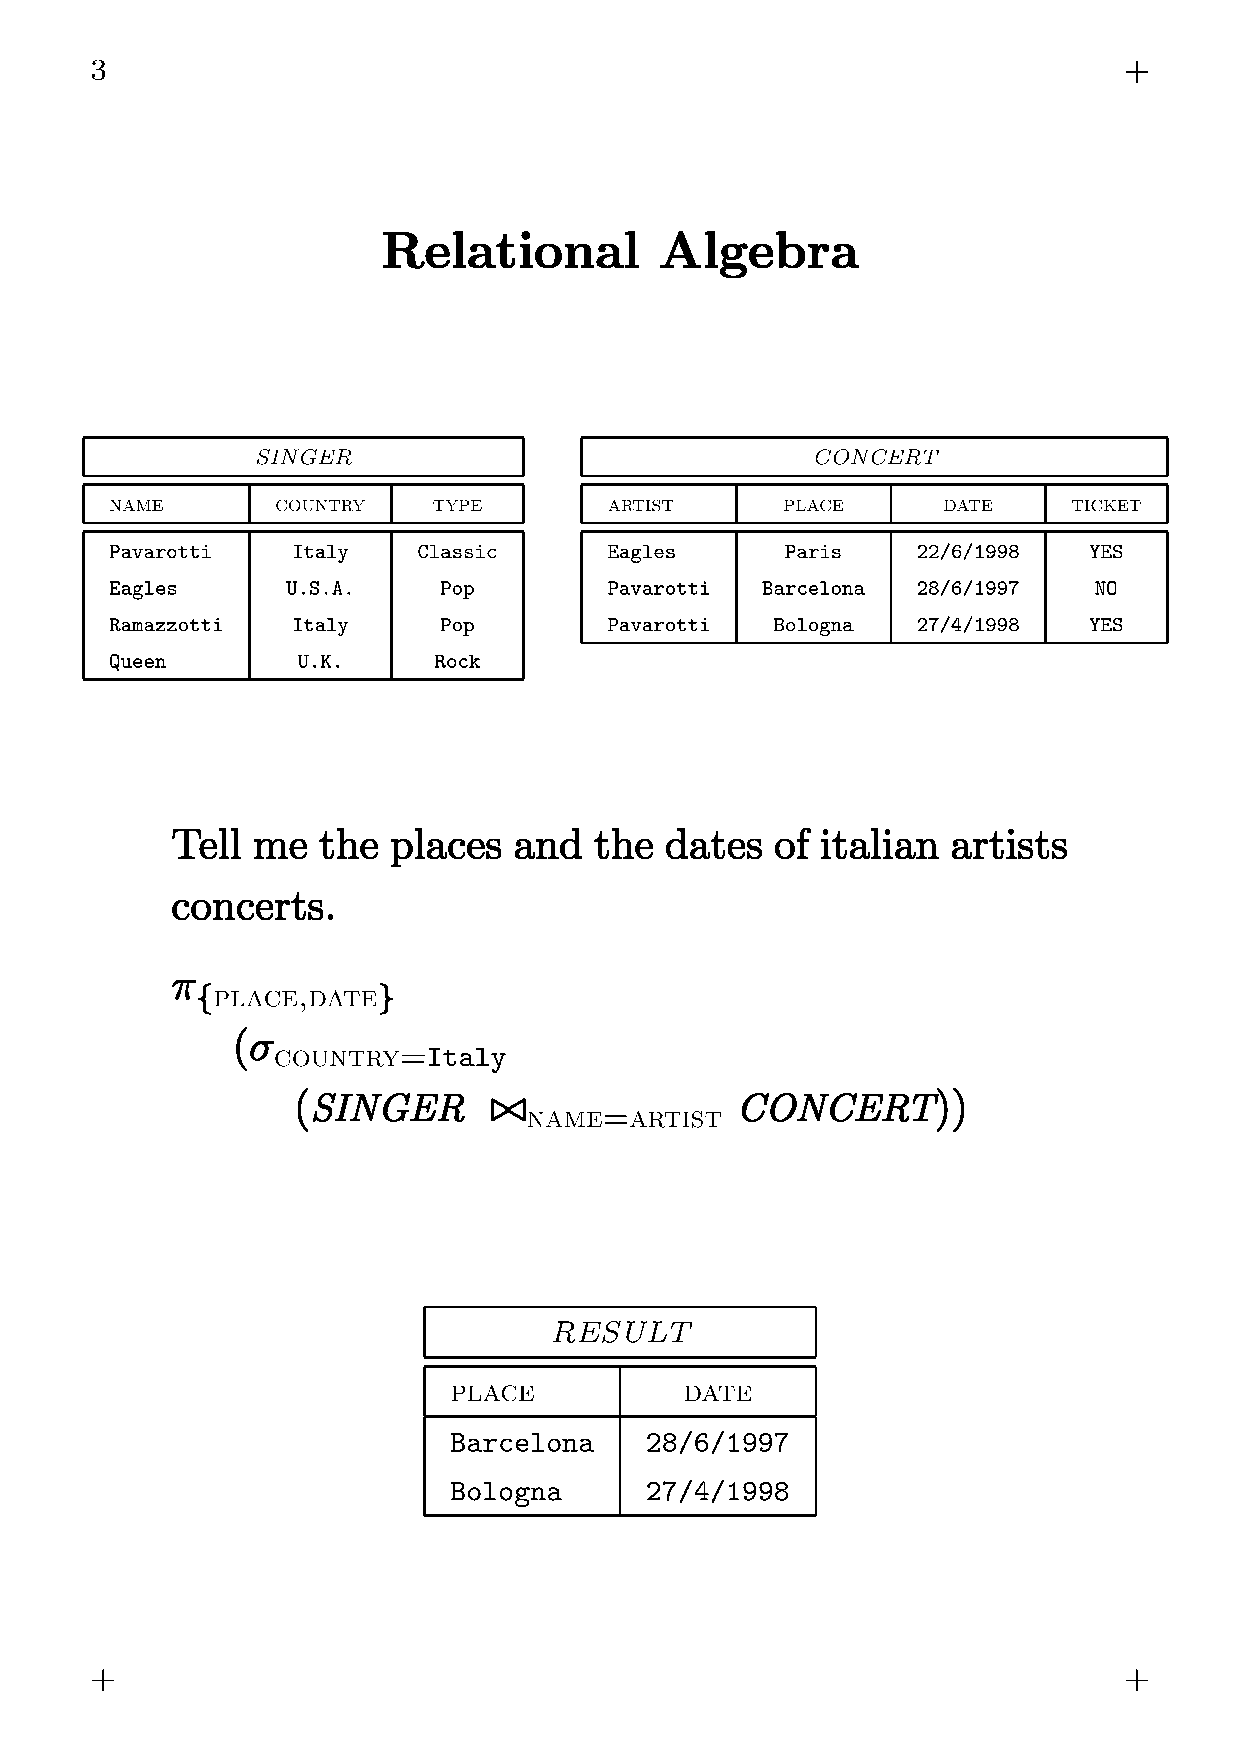
\includegraphics[width=0.95\linewidth]{relalg}
\end{slide*}

\begin{slide*}
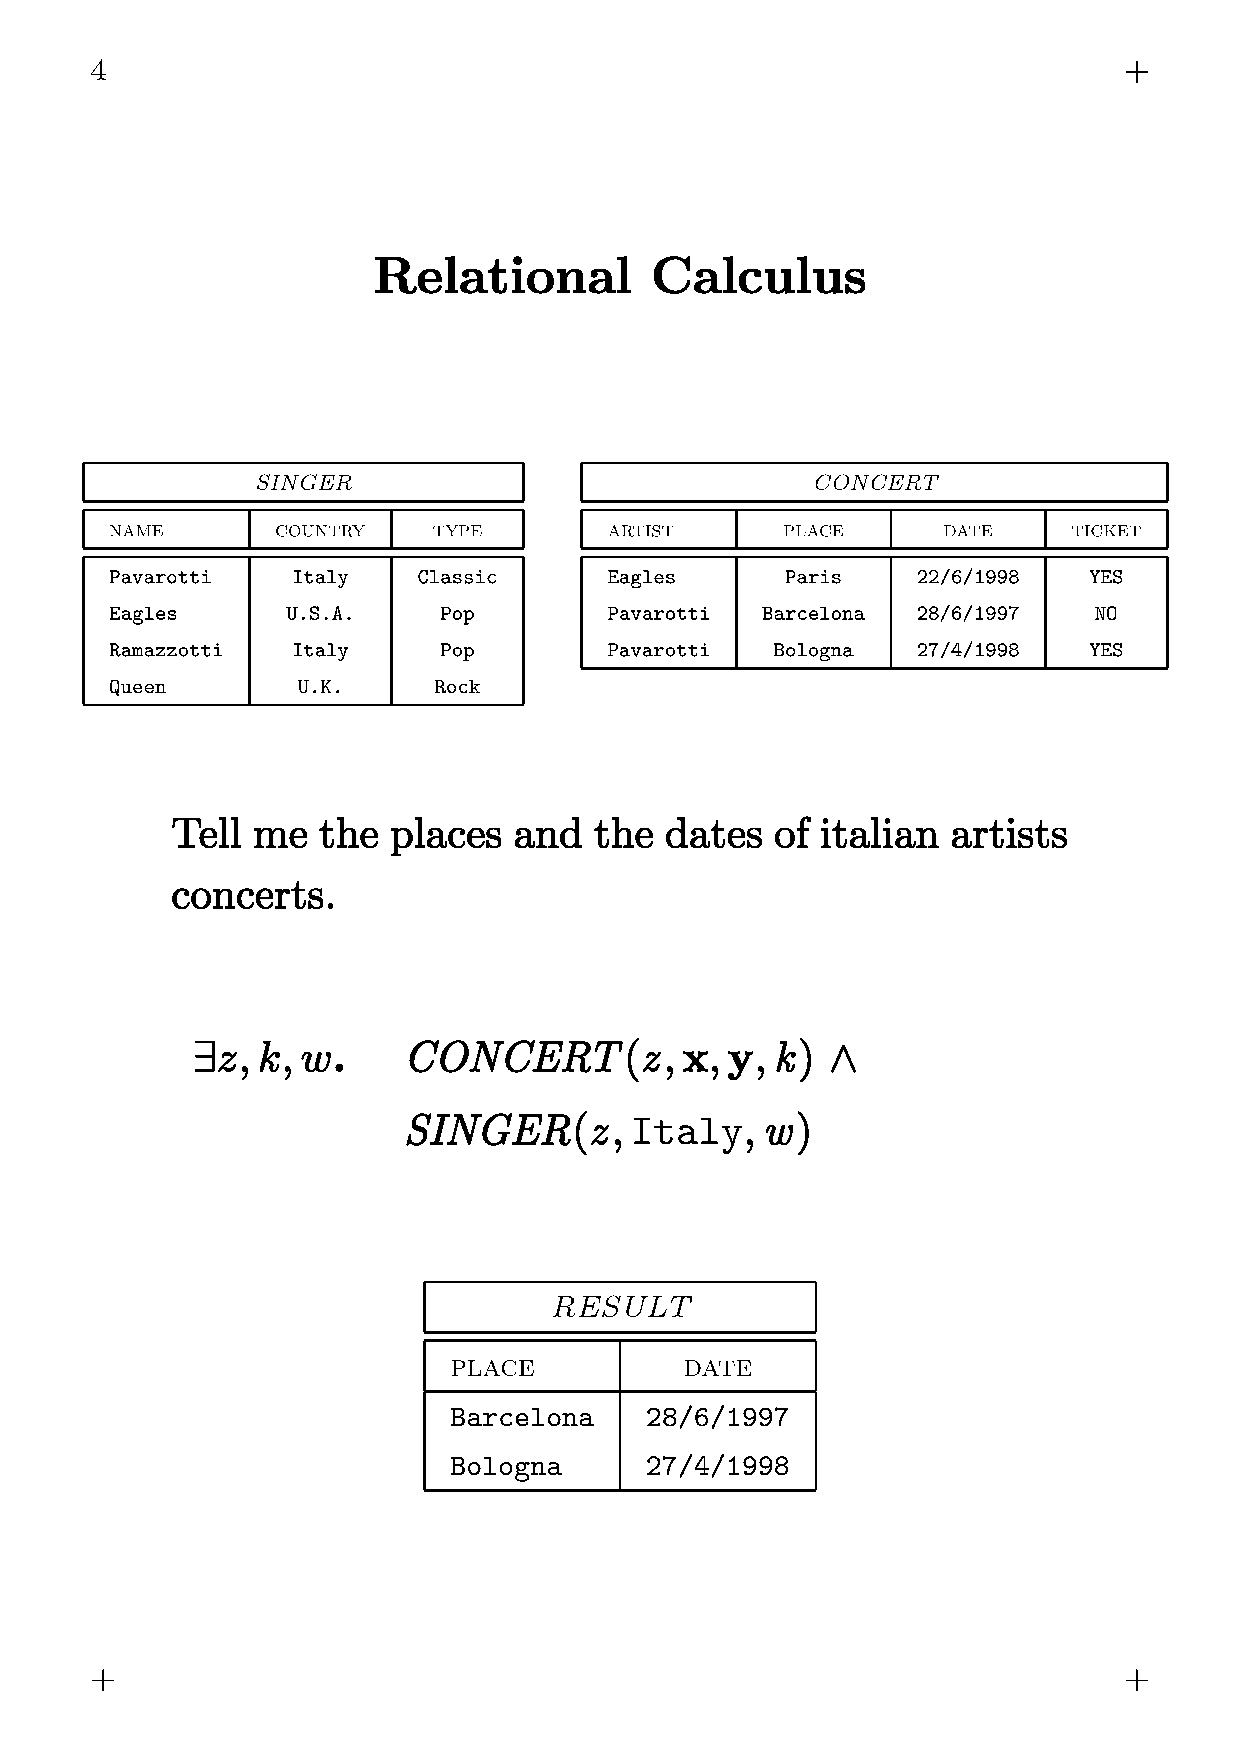
\includegraphics[width=0.95\linewidth]{relcalc}
\end{slide*}

\begin{slide*}
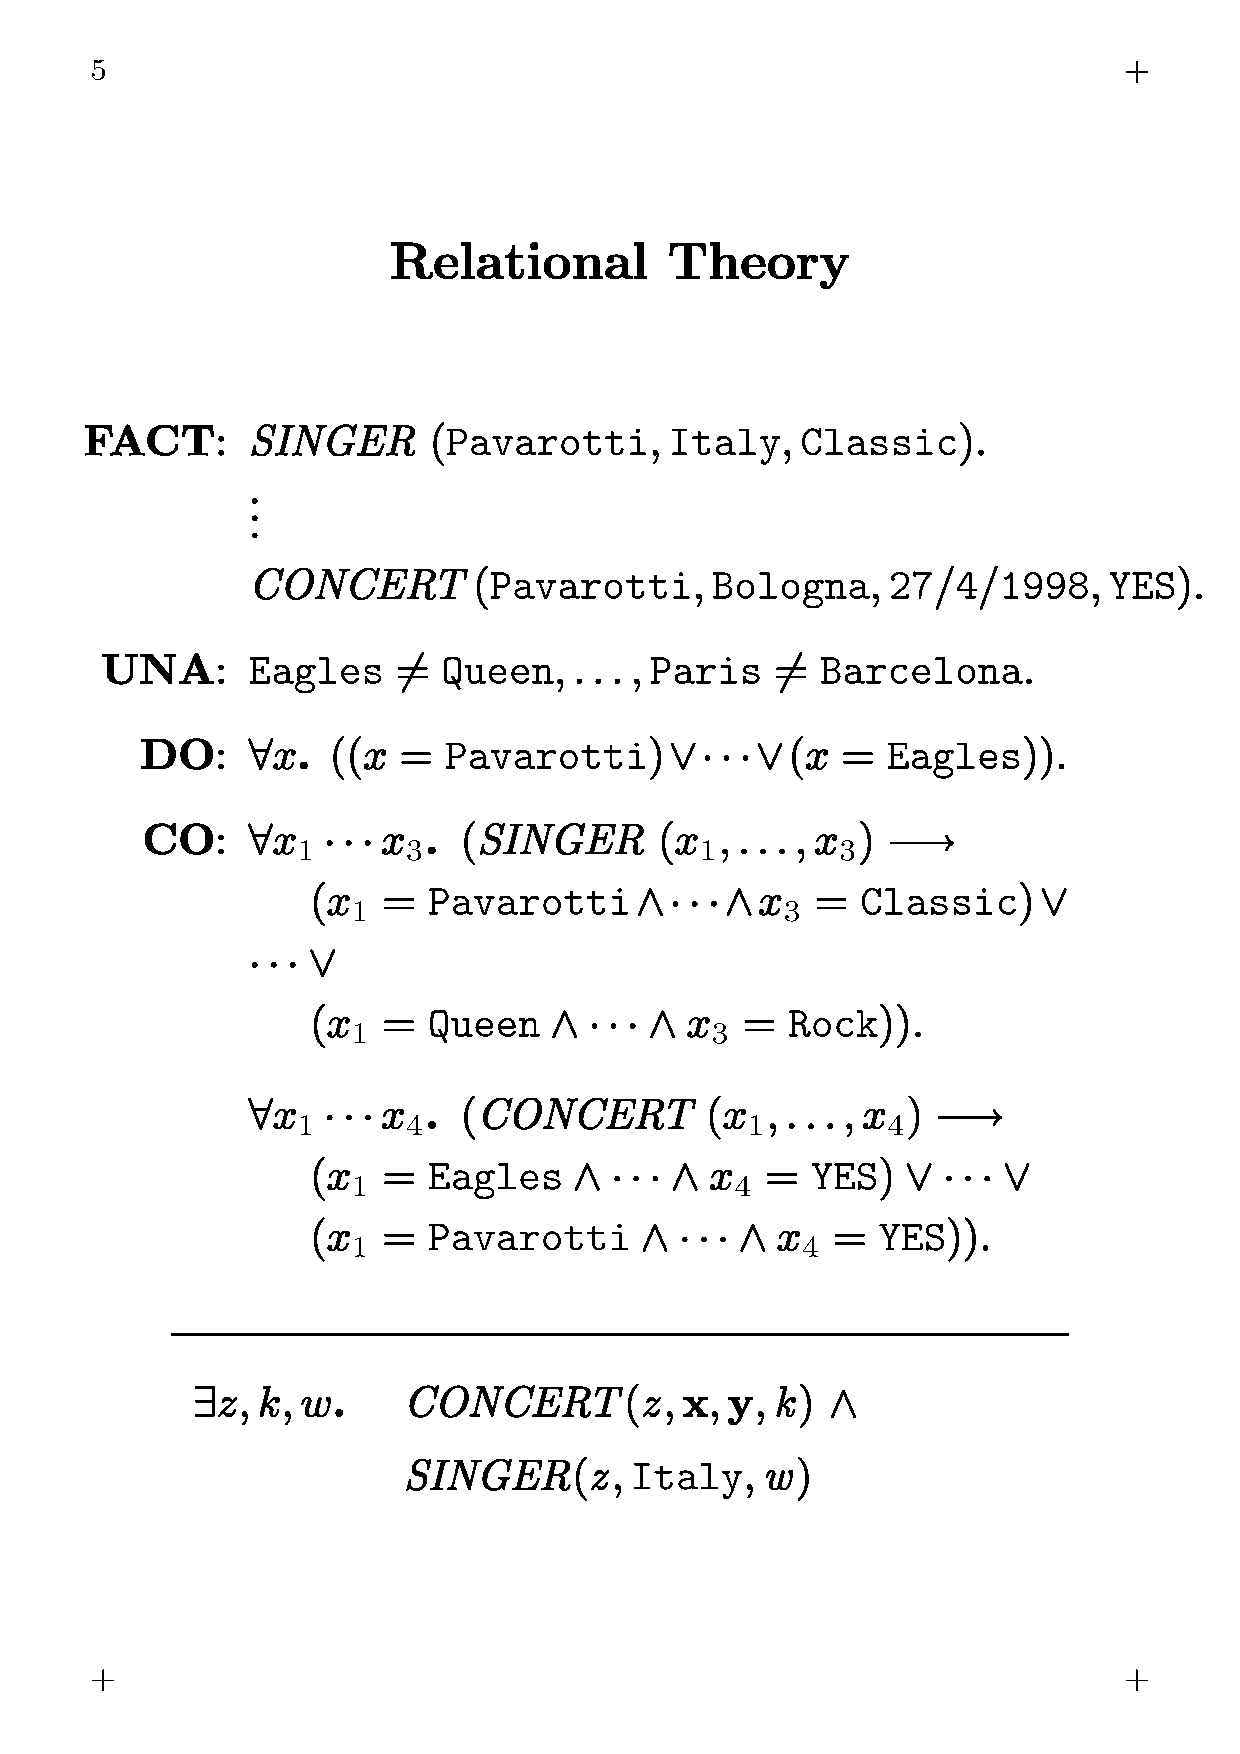
\includegraphics[width=0.95\linewidth]{reltheory}
\end{slide*}

\end{document}

%%% Local Variables: 
%%% mode: latex
%%% TeX-master: t
%%% End: 
